\documentclass[11pt,a4paper,twoside]{book}
\usepackage[utf8]{vietnam} 
%\usepackage{extsizes}
%\usepackage{amssymb,yhmath,mathrsfs,fontawesome}
%,amsmath,amssymb,fontawesome,txfonts,,txfonts}
\usepackage{amsmath,amssymb,yhmath,mathrsfs,fontawesome5,tcolorbox}
%Đổi font
\def\mautheme{green!40!black}
%\usepackage{bbm}
\let\widering\relax
%\usepackage[poorman]{fourier}
%\usepackage[T5]{fontenc}
%\usepackage{fouriernc}
\usepackage{fancyhdr}
\usepackage{enumerate}
\usepackage{tkz-euclide}
\usepackage{tikz-3dplot}
\usepackage{array}
\usepackage{tikz,tkz-tab}
\usetikzlibrary{shapes.geometric,arrows,calc,intersections,angles,quotes,patterns,positioning}
\usepackage{pgfplots}
\usepgfplotslibrary{fillbetween}
\pgfplotsset{compat=1.4}
\usepackage[top=1.5cm, bottom=1.5cm, left=1.5cm, right=1.5cm] {geometry}
\usepackage[hidelinks,unicode]{hyperref}
\usepackage{currfile}
\usepackage{hyperref}
\usepackage{eso-pic}

%\usepackage[dethi]{ex_test}
%\usepackage[loigiai]{ex_test}
%\usepackage[color]{ex_test}
\usepackage[solcolor,book]{ex_test}
%CÁC GÓI, LỆNH VIẾT TẮT CẦN THÊM
%\usepackage[poorman]{fourier}
%\usepackage[T5]{fontenc}
%\let\widering\relax % phu hợp font fourier
%\renewcommand{\baselinestretch}{1.1}
%CẤU TRÚC TỰ LUẬN
\usepackage{framed}


\newtheorem{bt}{\textbf{Câu}}
\newtheorem{vd}{\textbf{Ví dụ}}
\setcounter{bt}{0}
\setcounter{vd}{0}
\setcounter{subsubsection}{0}

\theorembodyfont{\rm}
\newtheorem{dl}{\fontfamily{ptm}\selectfont Định lí}
\theoremseparator{.}
\theorembodyfont{\rm}
\newtheorem{hq}{\fontfamily{ptm}\selectfont Hệ quả}
\newtheorem{tc}{\fontfamily{ptm}\selectfont Tính chất}
\newtheorem{dn}{\fontfamily{ptm}\selectfont Định nghĩa}
\theoremstyle{nonumberplain}
\newtheorem{kn}{\fontfamily{ptm}\selectfont Khái niệm}
\theoremseparator{}
\theorembodyfont{\it}
\usepackage{stackengine}
\usepackage{scalerel}
\newcommand\dangersign[1][2ex]{%
\renewcommand\stacktype{L}%
\scaleto{\stackon[1.3pt]{\color{red}$\triangle$}{\fontsize{4}{0}\selectfont !}}{#1}%
}
\newtheorem{note}{{\dangersign[3ex]}}
\newtheorem{nx}{Nhận xét.}

% =============================================================================
% PROOFDOT 2 CHE DO
% =============================================================================
% Dung:
%   \begin{proofdot}{6}{a}\end{proofdot}  -> dong cham mot cot nhu ban cu
%   \begin{proofdot}{6}{b}\end{proofdot}  -> dong cham chia doi, co vach doc giua
%VD1: đang cần các câu từ 3 đến 9, chỉ cần gõ \printEX{{3}{9}}.
%+ VD2: đang cần các câu từ 3 đến 9, rồi câu 25 đến 37, chỉ cần gõ \printEX{{3}{9}{25}{37}}.
%+ VD3: đang cần các câu từ 3 đến 9, câu 18, rồi câu 21 đến 32, chỉ cần gõ \printEX{{3}{9}{18}{18}{21}{32}}.

\newcommand{\TSATheoremProofDotA}[1]{%
  \multido{}{#1}{\noindent\makebox[\linewidth]{\dotfill}\\[6.5mm]}%
}

% Cập nhật chế độ A (dòng chấm ngang) để sử dụng TikZ với độ đậm lớn hơn
\renewcommand{\TSATheoremProofDotA}[1]{%
	\ifnum#1>0\relax
	\par\addvspace{2pt}%
	\noindent\begin{tikzpicture}[x=\linewidth,y=1cm]
		% Giãn dòng bằng chế độ B (hệ số 1.1)
		\pgfmathsetmacro{\TSAProofDotLast}{#1*1.1}
		\pgfmathsetmacro{\TSAProofDotBottom}{-\TSAProofDotLast-.18}
		\useasboundingbox (0,.12) rectangle (1,\TSAProofDotBottom);
		% Kẻ dòng chấm ngang ĐẬM
		\foreach \i in {1,...,#1}{%
			\pgfmathsetmacro{\yy}{-\i*1.1}
			% Màu đen đậm và độ dày lớn hơn (.7pt)
			\draw[black!85,line width=.7pt,densely dotted] (.02,\yy) -- (.98,\yy);
		}%
	\end{tikzpicture}%
	\par\addvspace{2pt}%
	\fi
}

% Cập nhật chế độ B (chia cột) với độ đậm lớn hơn và giãn dòng 1.1
\providecommand{\TSATheoremProofDotB}{}
\renewcommand{\TSATheoremProofDotB}[1]{%
	\ifnum#1>0\relax
	\par\addvspace{1pt}%
	\noindent\begin{tikzpicture}[x=\linewidth,y=1cm]
		% Hệ số giãn dòng 1.1
		\pgfmathsetmacro{\TSAProofDotLast}{#1*1.1}
		\pgfmathsetmacro{\TSAProofDotBottom}{-\TSAProofDotLast-.18}
		\useasboundingbox (0,.12) rectangle (1,\TSAProofDotBottom);
		% Kẻ vạch dọc ở giữa (vẫn giữ xám để làm hướng dẫn nhẹ)
		\draw[gray!60,line width=.85pt] (.5,-.16) -- (.5,-\TSAProofDotLast-.12);
		\foreach \i in {1,...,#1}{%
			\pgfmathsetmacro{\yy}{-\i*1.1}
			% Màu đen đậm và độ dày lớn hơn (.7pt) cho các dòng chấm
			\draw[black!85,line width=.7pt,densely dotted] (.02,\yy) -- (.47,\yy);
			\draw[black!85,line width=.7pt,densely dotted] (.53,\yy) -- (.98,\yy);
		}%
	\end{tikzpicture}%
	\par\addvspace{2pt}%
	\fi
}

\newif\ifTSATheoremProofDotSplit
\newcommand{\TSATheoremProofDotSelect}[2]{%
  \TSATheoremProofDotSplitfalse
  \def\TSAProofDotMode{#2}%
  \def\TSAProofDotModeb{b}%
  \def\TSAProofDotModeB{B}%
  \ifx\TSAProofDotMode\TSAProofDotModeb\TSATheoremProofDotSplittrue\fi
  \ifx\TSAProofDotMode\TSAProofDotModeB\TSATheoremProofDotSplittrue\fi
  \ifTSATheoremProofDotSplit
    \TSATheoremProofDotB{#1}%
  \else
    \TSATheoremProofDotA{#1}%
  \fi
}

\makeatletter
% =============================================================================
% KIỂM TRA CHẾ ĐỘ ẨN / HIỆN CỦA PROOFDOT
% Tự động ẩn khi bật 1 trong 3 tùy chọn: loigiai, color, solcolor của ex_test
% =============================================================================
\newif\ifTSAHideProofDot
\def\TSAProofDotOverride{-1}% -1: tự động, 0: luôn hiện, 1: luôn ẩn
\newcommand{\HideProofDot}{\def\TSAProofDotOverride{1}}
\newcommand{\ShowProofDot}{\def\TSAProofDotOverride{0}}
\newcommand{\AutoProofDot}{\def\TSAProofDotOverride{-1}}

\newcommand{\TSACheckProofDotHide}{%
  \ifnum\TSAProofDotOverride=1\relax
    \TSAHideProofDottrue
  \else\ifnum\TSAProofDotOverride=0\relax
    \TSAHideProofDotfalse
  \else
    \TSAHideProofDotfalse
    % 1. Kiểm tra cờ \if@extest@hasanykey của ex_test (bật khi dùng loigiai, color, solcolor)
    \ifdefined\if@extest@hasanykey
      \if@extest@hasanykey \TSAHideProofDottrue \fi
    \fi
    % 2. Kiểm tra chuỗi tùy chọn \kindOPTN (loigiai, color, solcolor)
    \ifdefined\kindOPTN
      \IfSubStrEX{,solcolor,loigiai,color,}{,\kindOPTN,}{\TSAHideProofDottrue}{}%
    \fi
    % 3. Kiểm tra các cờ hiển thị lời giải / màu sắc
    \ifdefined\if@extest@showloigiai
      \if@extest@showloigiai \TSAHideProofDottrue \fi
    \fi
    \ifdefined\if@extest@showcolor
      \if@extest@showcolor \TSAHideProofDottrue \fi
    \fi
  \fi\fi
}

\DeclareDocumentEnvironment{proofdot}{m g +b}{%
  \TSACheckProofDotHide
  \ifTSAHideProofDot
    % Tự giác %: Ẩn hoàn toàn, không in dòng kẻ chấm hay sinh ra khoảng cách thừa
  \else
    % Chế độ in đề (dethi, book,...): In các dòng kẻ chấm
    \par\addvspace{-4pt}%
    \IfNoValueTF{#2}{\TSATheoremProofDotSelect{#1}{a}}{\TSATheoremProofDotSelect{#1}{#2}}%
    \par\addvspace{.5\topsep}%
  \fi
}{}
\makeatother
%%%%%
%Xài ký hiệu không chia hết, chia hết
\def\kch{\mathrel{\ooalign{$\vdots$\cr\hidewidth$\raisebox{0.25ex}{$/$}$\hidewidth\cr}}}
\def\ch{\mathrel{\vdots}}

%Tiêu đề chương
\setcounter{secnumdepth}{4}
\setcounter{tocdepth}{2}
\usepackage{titlesec}
\usepackage{titletoc}
%Làm mục lục
%\patchcmd{\tableofcontents}{\contentsname}{\color{black}MỤC LỤC}{}{}
\usepackage{ifoddpage}
\titlecontents{section}
[4em]{\sffamily}
{\color{black}\contentslabel{2.3em}\color{black}}{}
{\titlerule*[1000pc]{.}\contentspage\\\hspace*{-3em}\vspace*{2pt}%
\color{black}\rule{\dimexpr\textwidth-16pt\relax}{1pt}}

\titlecontents{lsection}
[5.8em]{\sffamily}
{\color{black}\contentslabel{2.3em}\color{black}}{}
{\titlerule*[1000pc]{.}\contentspage\\\hspace*{-5.8em}\vspace*{2pt}%
\color{black}\rule{\dimexpr\textwidth\relax}{1pt}}

\renewcommand\thesection{\@arabic\c@section}
\renewcommand\thesubsection{\@Alph\c@subsection}
\renewcommand\thesubsubsection{\@arabic\c@subsubsection}


\usepackage{esvect}
\def\vec{\vv}
\def\overrightarrow{\vv}

\usepackage{lastpage}
\pagestyle{fancy}
\fancyhf{} 
\renewcommand{\headrulewidth}{0pt}
%\lfoot{\it\sf\fontsize{12pt}{1pt}\selectfont\faMortarBoard\, \nouppercase{\color{red!70!black}NoadDVo}}
%\rfoot{\sf\fontsize{12pt}{1pt}\selectfont\faClockO\, \color{red!70!black}Trang~\thepage/\pageref{LastPage}}
%\newpage
%\chead{\empty}
%\rhead{\it\sf\nouppercase{\fontsize{10pt}{1pt}\selectfont\faIcon{envelope}\color{red!70!black}\ dangnguyen402042@gmail.com}}
%\lhead{\sf\fontsize{10pt}{1pt}\selectfont\faFileText\,\color{red!70!black}~ĐỀ THI TỐT NGHIỆP THPT 2026 -- LẦN 2}
%HẾT CẤU TRÚC TỰ LUẬN
\newcommand{\hoac}[1]{\left[\begin{aligned}#1\end{aligned}\right.}
\newcommand{\heva}[1]{\left\{\begin{aligned}#1\end{aligned}\right.}
\renewcommand\loigiaiEX {\color{black} Lời giải}
\renewcommand{\baselinestretch}{1.25}
\renewcommand{\labelenumi}{\alph{enumi})}
%dấu chấm đậm
\renewcommand{\TrueEX}{\stepcounter{dapan}{\textbf{\color{black}\Alph{dapan}.}} \ignorespaces}
\renewcommand{\FalseEX}{\stepcounter{dapan}{\textbf{\color{black}\Alph{dapan}.}} \ignorespaces}

\newcommand{\caulc}{
	\begin{flushleft}
		{\color{\mautheme} \textbf{PHẦN I. Câu trắc nghiệm nhiều phương án lựa chọn.} Thí sinh trả lời từ câu 1 đến câu 12. Mỗi câu hỏi thí sinh chỉ chọn một phương án.}
	\end{flushleft}
	\setcounter{ex}{0}
}
\newcommand{\cauds}{
	{\color{\mautheme} \noindent\textbf{PHẦN II. Câu trắc nghiệm đúng sai.} Thí sinh trả lời từ câu 1 đến câu 4. Trong mỗi ý \textbf{a)}, \textbf{b)}, \textbf{c)}, \textbf{d)} ở mỗi câu, thí sinh chọn đúng hoặc sai.}
	\setcounter{ex}{0}
}
\newcommand{\caukq}{
	\begin{flushleft}
		{\color{\mautheme} \noindent\textbf{PHẦN III. Câu trắc nghiệm trả lời ngắn.} Thí sinh trả lời từ câu 1 đến câu 6.}
	\end{flushleft}
	\setcounter{ex}{0}
}
\newcommand{\tl}{
	\begin{flushleft}
		{\color{\mautheme} \noindent\textbf{PHẦN IV. Tự luận.}}
	\end{flushleft}
	\setcounter{bt}{0}
}
\makeatother
\newcommand{\indapan}[2]{
\inputansbox{#1}{#2}
}
\newcommand{\AnBangdapan}{
\renewcommand{\indapan}[2]{}
}
% ==========================
% PDF FINGERPRINT
% ==========================
\newcommand{\PDFFingerprint}{NDV-402042}

\hypersetup{
	pdfkeywords={NoadD,\PDFFingerprint}
}
%\printEX[1,...,5,8,,23,...,29]{ex}

\begin{document}
\def\tacgia{\bf KIỂM TRA THƯỜNG XUYÊN}

\everymath{\displaystyle}

% ==============================================================================
% ĐỀ KIỂM TRA GIỮA HỌC KÌ I - MÔN TOÁN 6 - ĐỀ 1
% ==============================================================================

\noindent
\begin{minipage}[t]{6.5cm}
	\centering
	\textbf{TRƯỜNG THCS \dots\dots\dots\dots\dots\dots}\\[3pt]
	\textbf{TỔ: \dots\dots\dots\dots\dots\dots}\\[6pt]
	\textbf{(ĐỀ 1)}\\
	(\textit{Đề có 02 trang})
\end{minipage}%
\hfill
\begin{minipage}[t]{10.5cm}
	\centering
	\textbf{ĐỀ KIỂM TRA GIỮA HỌC KÌ I}\\[3pt]
	\textbf{NĂM HỌC 2026 -- 2027}\\[3pt]
	\textbf{Môn: TOÁN -- Lớp 6}\\[3pt]
	\textit{Thời gian làm bài: 90 phút (không kể thời gian giao đề)}
\end{minipage}

\vspace{10pt}

\noindent
\textbf{Họ và tên học sinh:} \dotfill{} \textbf{Lớp:} \makebox[2.5cm]{\dotfill} \textbf{Số báo danh:} \makebox[2.5cm]{\dotfill}

\vspace{10pt}

% ------------------------------------------------------------------------------
% PHẦN I: TRẮC NGHIỆM NHIỀU PHƯƠNG ÁN LỰA CHỌN
% ------------------------------------------------------------------------------
\noindent\textbf{PHẦN I. Câu trắc nghiệm nhiều phương án lựa chọn (3,0 điểm).}\\
\textit{Thí sinh trả lời từ câu 1 đến câu 12. Mỗi câu hỏi thí sinh chỉ chọn một phương án.}

\setcounter{ex}{0}

\begin{ex}%Câu 1
	Cho tập hợp $A = \{2; 4; 6; 8\}$. Khẳng định nào sau đây đúng?
	\choice
	{$3 \in A$}
	{$8 \notin A$}
	{\True $6 \in A$}
	{$5 \in A$}
	\loigiai{
		Phần tử $6$ thuộc tập hợp $A$ nên khẳng định đúng là $6 \in A$.
	}
\end{ex}

\begin{ex}%Câu 2
	Trong số $4\,527$, chữ số $5$ có giá trị là
	\choice
	{\True $500$}
	{$50$}
	{$5$}
	{$5\,000$}
	\loigiai{
		Chữ số $5$ nằm ở hàng trăm nên có giá trị là $500$.
	}
\end{ex}

\begin{ex}%Câu 3
	Số tự nhiên liền sau của số $2\,099$ là
	\choice
	{$2\,098$}
	{$2\,009$}
	{$3\,000$}
	{\True $2\,100$}
	\loigiai{
		Số tự nhiên liền sau của số $2\,099$ là $2\,099 + 1 = 2\,100$.
	}
\end{ex}

\begin{ex}%Câu 4
	Kết quả của phép tính $3^4 \cdot 3^2$ viết dưới dạng một luỹ thừa là
	\choice
	{$3^8$}
	{\True $3^6$}
	{$9^6$}
	{$3^2$}
	\loigiai{
		Áp dụng quy tắc nhân hai luỹ thừa cùng cơ số: $3^4 \cdot 3^2 = 3^{4+2} = 3^6$.
	}
\end{ex}

\begin{ex}%Câu 5
	Đối với biểu thức không có dấu ngoặc, gồm các phép tính cộng, trừ, nhân, chia, nâng lên luỹ thừa, thứ tự thực hiện phép tính là
	\choice
	{Nhân và chia, rồi đến nâng lên luỹ thừa, cuối cùng đến cộng và trừ}
	{Cộng và trừ, rồi đến nhân và chia, cuối cùng đến nâng lên luỹ thừa}
	{\True Nâng lên luỹ thừa, rồi đến nhân và chia, cuối cùng đến cộng và trừ}
	{Thực hiện lần lượt từ trái sang phải, không phân biệt loại phép tính}
	\loigiai{
		Thứ tự thực hiện phép tính: Luỹ thừa $\to$ Nhân và chia $\to$ Cộng và trừ.
	}
\end{ex}

\begin{ex}%Câu 6
	Số nào sau đây là ước của $18$?
	\choice
	{\True $6$}
	{$4$}
	{$36$}
	{$12$}
	\loigiai{
		Vì $18 \ \vdots \ 6$ nên $6$ là ước của $18$.
	}
\end{ex}

\begin{ex}%Câu 7
	Số nào sau đây chia hết cho cả $2$ và $5$?
	\choice
	{$1\,235$}
	{\True $1\,230$}
	{$1\,232$}
	{$2\,025$}
	\loigiai{
		Số chia hết cho cả $2$ và $5$ có chữ số tận cùng bằng $0$, do đó chọn $1\,230$.
	}
\end{ex}

\begin{ex}%Câu 8
	Số nào sau đây là số nguyên tố?
	\choice
	{$15$}
	{$21$}
	{$1$}
	{\True $13$}
	\loigiai{
		Số $13$ chỉ có hai ước tự nhiên là $1$ và $13$ nên là số nguyên tố.
	}
\end{ex}

\begin{ex}%Câu 9
	Tập hợp $\text{ƯC}(6, 9)$ là
	\choice
	{\True $\{1; 3\}$}
	{$\{1; 2; 3\}$}
	{$\{3\}$}
	{$\{1; 3; 6; 9\}$}
	\loigiai{
		Ta có $\text{Ư}(6) = \{1; 2; 3; 6\}$ và $\text{Ư}(9) = \{1; 3; 9\}$. Do đó $\text{ƯC}(6, 9) = \{1; 3\}$.
	}
\end{ex}

\begin{ex}%Câu 10
	Kết quả phân tích số $120$ ra thừa số nguyên tố là
	\choice
	{$2^2 \cdot 3 \cdot 10$}
	{$2^3 \cdot 15$}
	{\True $2^3 \cdot 3 \cdot 5$}
	{$2 \cdot 3 \cdot 4 \cdot 5$}
	\loigiai{
		Ta có $120 = 8 \cdot 15 = 2^3 \cdot 3 \cdot 5$.
	}
\end{ex}

\begin{ex}%Câu 11
	\noindent
	\begin{minipage}[t]{0.70\linewidth}
		Cho hình chữ nhật $ABCD$ có hai đường chéo cắt nhau tại $O$ (hình bên). Khẳng định nào sau đây đúng?
		\choice
		{$AB = BC$}
		{\True $AC = BD$}
		{$AC \perp BD$}
		{$OA = AB$}
	\end{minipage}\hfill
	\begin{minipage}[t]{0.26\linewidth}
		\centering\vspace{0pt}
		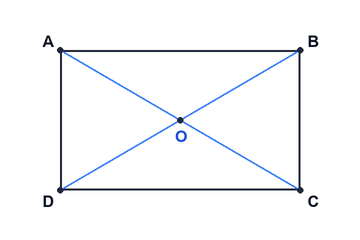
\includegraphics[width=\linewidth]{images/de1_cau11.png}
	\end{minipage}
	\loigiai{
		Trong hình chữ nhật, hai đường chéo bằng nhau. Do đó khẳng định đúng là $AC = BD$.
	}
\end{ex}

\begin{ex}%Câu 12
	\noindent
	\begin{minipage}[t]{0.70\linewidth}
		Hình thoi $MNPQ$ ở hình bên có hai đường chéo $MP = 8\text{ cm}$, $NQ = 6\text{ cm}$. Diện tích hình thoi $MNPQ$ là
		\choice
		{$48\text{ cm}^2$}
		{$14\text{ cm}^2$}
		{$28\text{ cm}^2$}
		{\True $24\text{ cm}^2$}
	\end{minipage}\hfill
	\begin{minipage}[t]{0.26\linewidth}
		\centering\vspace{0pt}
		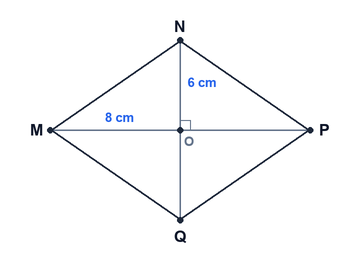
\includegraphics[width=\linewidth]{images/de1_cau12.png}
	\end{minipage}
	\loigiai{
		Diện tích hình thoi bằng nửa tích độ dài hai đường chéo:
		\[ S = \frac{1}{2} \cdot 8 \cdot 6 = 24\text{ (cm}^2\text{)}. \]
	}
\end{ex}

\vspace{8pt}

% ------------------------------------------------------------------------------
% PHẦN II: CÂU TRẮC NGHIỆM ĐÚNG SAI
% ------------------------------------------------------------------------------
\noindent\textbf{PHẦN II. Câu trắc nghiệm đúng sai (2,0 điểm).}\\
\textit{Thí sinh trả lời từ câu 13 đến câu 14. Trong mỗi ý a), b), c), d) ở mỗi câu, thí sinh chọn đúng hoặc sai.}

\begin{ex}%Câu 13
	Cho hai số $a = 72$ và $b = 108$.
	\choiceTF
	{\True $a$ chia hết cho $9$}
	{$b$ là số nguyên tố}
	{\True $\text{ƯCLN}(a, b) = 36$}
	{Có đúng $4$ bội chung khác $0$ của $a$ và $b$ nhỏ hơn $700$}
	\loigiai{
		\begin{itemchoice}
			\item Đúng: $7 + 2 = 9$ chia hết cho $9$ nên $72 \ \vdots \ 9$.
			\item Sai: $108$ có chữ số tận cùng là $8$ nên chia hết cho $2$ (có các ước khác $1$ và chính nó), do đó $b$ là hợp số.
			\item Đúng: Phân tích ra thừa số nguyên tố: $72 = 2^3 \cdot 3^2$ và $108 = 2^2 \cdot 3^3$. Suy ra $\text{ƯCLN}(a, b) = 2^2 \cdot 3^2 = 36$.
			\item Sai: $\text{BCNN}(a, b) = 2^3 \cdot 3^3 = 216$. Các bội chung khác $0$ của $a$ và $b$ nhỏ hơn $700$ là: $216; 432; 648$, chỉ có $3$ số.
		\end{itemchoice}
	}
\end{ex}

\begin{ex}%Câu 14
	\noindent
	\begin{minipage}[t]{0.68\linewidth}
		Một mảnh bìa hình chữ nhật $ABCD$ có $AB = 10\text{ cm}$, $BC = 6\text{ cm}$. Trên cạnh $AB$ lấy điểm $E$, trên cạnh $CD$ lấy điểm $F$ sao cho $AE = DF = 4\text{ cm}$ (hình bên).
		\choiceTF
		{\True $CD = 10\text{ cm}$}
		{Hình chữ nhật $ABCD$ có hai đường chéo vuông góc với nhau}
		{\True Diện tích tứ giác $EBCF$ bằng $36\text{ cm}^2$}
		{\True Cắt mảnh bìa theo đoạn thẳng $EF$ được hai mảnh. Tổng chu vi hai mảnh lớn hơn chu vi mảnh bìa ban đầu là $12\text{ cm}$}
	\end{minipage}\hfill
	\begin{minipage}[t]{0.28\linewidth}
		\centering\vspace{0pt}
		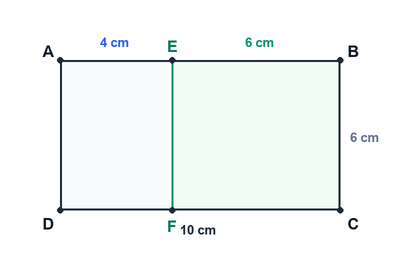
\includegraphics[width=\linewidth]{images/de1_cau14.png}
	\end{minipage}
	\loigiai{
		\begin{itemchoice}
			\item Đúng: Trong hình chữ nhật, các cạnh đối bằng nhau nên $CD = AB = 10\text{ cm}$.
			\item Sai: Hình chữ nhật có hai đường chéo bằng nhau; vì $AB \neq BC$ nên hai đường chéo không vuông góc với nhau.
			\item Đúng: Ta có $EB = AB - AE = 10 - 4 = 6\text{ cm}$ và $FC = CD - DF = 10 - 4 = 6\text{ cm}$. Tứ giác $EBCF$ là hình vuông cạnh $6\text{ cm}$ nên có diện tích $6 \cdot 6 = 36\text{ cm}^2$.
			\item Đúng: Chu vi hình chữ nhật $AEFD$ là $(4 + 6) \cdot 2 = 20\text{ cm}$; chu vi hình vuông $EBCF$ là $4 \cdot 6 = 24\text{ cm}$. Chu vi hình chữ nhật ban đầu $ABCD$ là $(10 + 6) \cdot 2 = 32\text{ cm}$. Tổng chu vi hai mảnh lớn hơn chu vi ban đầu là: $20 + 24 - 32 = 12\text{ cm}$ (chính bằng $2 \cdot EF = 2 \cdot 6 = 12\text{ cm}$).
		\end{itemchoice}
	}
\end{ex}

\vspace{8pt}

% ------------------------------------------------------------------------------
% PHẦN III: CÂU TRẮC NGHIỆM TRẢ LỜI NGẮN
% ------------------------------------------------------------------------------
\noindent\textbf{PHẦN III. Câu trắc nghiệm trả lời ngắn (2,0 điểm).}\\
\textit{Thí sinh trả lời từ câu 15 đến câu 18.}

\begin{ex}%Câu 15
	Tính giá trị của biểu thức $2^5 - 5^2$.
	\shortans{7}
	\loigiai{
		$2^5 - 5^2 = 32 - 25 = 7$.
	}
\end{ex}

\begin{ex}%Câu 16
	Tìm chữ số $x$ để số $\overline{25x}$ chia hết cho cả $3$ và $5$.
	\shortans{5}
	\loigiai{
		Vì $\overline{25x}$ chia hết cho $5$ nên $x \in \{0; 5\}$.
		\begin{itemize}
			\item Với $x = 0$, tổng các chữ số là $2 + 5 + 0 = 7$ không chia hết cho $3$.
			\item Với $x = 5$, tổng các chữ số là $2 + 5 + 5 = 12$ chia hết cho $3$.
		\end{itemize}
		Vậy chữ số cần tìm là $x = 5$.
	}
\end{ex}

\begin{ex}%Câu 17
	\noindent
	\begin{minipage}[t]{0.70\linewidth}
		Hình bình hành $ABCD$ ở hình bên có cạnh $CD = 9\text{ cm}$, chiều cao $AH = 5\text{ cm}$. Tính diện tích hình bình hành $ABCD$ (đơn vị: $\text{cm}^2$).
		\shortans{45}
	\end{minipage}\hfill
	\begin{minipage}[t]{0.26\linewidth}
		\centering\vspace{0pt}
		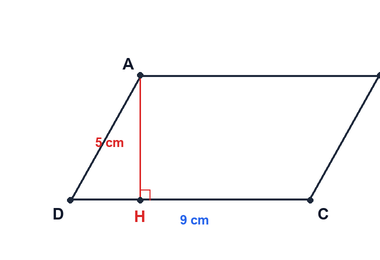
\includegraphics[width=\linewidth]{images/de1_cau17.png}
	\end{minipage}
	\loigiai{
		Diện tích hình bình hành $ABCD$ là:
		\[ S = CD \cdot AH = 9 \cdot 5 = 45\text{ (cm}^2\text{)}. \]
	}
\end{ex}

\begin{ex}%Câu 18
	Bạn Minh mua $5$ quyển vở, giá $12\,000$ đồng một quyển và $3$ chiếc bút bi, giá $8\,000$ đồng một chiếc. Minh đưa cho người bán tờ $100\,000$ đồng. Hỏi người bán phải trả lại Minh bao nhiêu nghìn đồng?
	\shortans{16}
	\loigiai{
		Tổng số tiền Minh phải trả là:
		\[ 5 \cdot 12\,000 + 3 \cdot 8\,000 = 60\,000 + 24\,000 = 84\,000\text{ (đồng)}. \]
		Số tiền người bán phải trả lại cho Minh là:
		\[ 100\,000 - 84\,000 = 16\,000\text{ (đồng)}, \]
		tức là $16$ nghìn đồng.
	}
\end{ex}



\clearpage
\setcounter{page}{1}
% ==============================================================================
% ĐỀ KIỂM TRA GIỮA HỌC KÌ I - MÔN TOÁN 6 - ĐỀ 2
% ==============================================================================

\noindent
\begin{minipage}[t]{6.5cm}
	\centering
	\textbf{TRƯỜNG THCS \dots\dots\dots\dots\dots\dots}\\[3pt]
	\textbf{TỔ: \dots\dots\dots\dots\dots\dots}\\[6pt]
	\textbf{(ĐỀ 2)}\\
	(\textit{Đề có 02 trang})
\end{minipage}%
\hfill
\begin{minipage}[t]{10.5cm}
	\centering
	\textbf{ĐỀ KIỂM TRA GIỮA HỌC KÌ I}\\[3pt]
	\textbf{NĂM HỌC 2026 -- 2027}\\[3pt]
	\textbf{Môn: TOÁN -- Lớp 6}\\[3pt]
	\textit{Thời gian làm bài: 90 phút (không kể thời gian giao đề)}
\end{minipage}

\vspace{10pt}

\noindent
\textbf{Họ và tên học sinh:} \dotfill{} \textbf{Lớp:} \makebox[2.5cm]{\dotfill} \textbf{Số báo danh:} \makebox[2.5cm]{\dotfill}

\vspace{10pt}

% ------------------------------------------------------------------------------
% PHẦN I: TRẮC NGHIỆM NHIỀU PHƯƠNG ÁN LỰA CHỌN
% ------------------------------------------------------------------------------
\noindent\textbf{PHẦN I. Câu trắc nghiệm nhiều phương án lựa chọn (3,0 điểm).}\\
\textit{Thí sinh trả lời từ câu 1 đến câu 12. Mỗi câu hỏi thí sinh chỉ chọn một phương án.}

\setcounter{ex}{0}

\begin{ex}%Câu 1
	Cho tập hợp $B = \{x \in \mathbb{N} \mid x < 4\}$. Viết tập hợp $B$ bằng cách liệt kê các phần tử, ta được
	\choice
	{$B = \{1; 2; 3\}$}
	{\True $B = \{0; 1; 2; 3\}$}
	{$B = \{0; 1; 2; 3; 4\}$}
	{$B = \{1; 2; 3; 4\}$}
	\loigiai{
		Các số tự nhiên nhỏ hơn $4$ gồm có $0; 1; 2; 3$, do đó $B = \{0; 1; 2; 3\}$.
	}
\end{ex}

\begin{ex}%Câu 2
	Số La Mã $\mathrm{XIV}$ có giá trị là
	\choice
	{$16$}
	{$9$}
	{$104$}
	{\True $14$}
	\loigiai{
		Trong hệ chữ số La Mã: $\mathrm{X} = 10$, $\mathrm{IV} = 4$. Do đó $\mathrm{XIV} = 10 + 4 = 14$.
	}
\end{ex}

\begin{ex}%Câu 3
	Số nhỏ nhất trong tập hợp $\mathbb{N}^*$ là
	\choice
	{\True $1$}
	{$0$}
	{$2$}
	{Không có số nhỏ nhất}
	\loigiai{
		Tập hợp $\mathbb{N}^* = \{1; 2; 3; \dots\}$, số nhỏ nhất trong tập hợp này là $1$.
	}
\end{ex}

\begin{ex}%Câu 4
	Kết quả của phép tính $5^7 : 5^3$ viết dưới dạng một luỹ thừa là
	\choice
	{$5^{10}$}
	{$5^{21}$}
	{\True $5^4$}
	{$1^4$}
	\loigiai{
		Áp dụng quy tắc chia hai luỹ thừa cùng cơ số: $5^7 : 5^3 = 5^{7 - 3} = 5^4$.
	}
\end{ex}

\begin{ex}%Câu 5
	Giá trị của biểu thức $20 - 2 \cdot 3^2$ là
	\choice
	{$162$}
	{\True $2$}
	{$14$}
	{$4$}
	\loigiai{
		Thực hiện luỹ thừa trước: $20 - 2 \cdot 3^2 = 20 - 2 \cdot 9 = 20 - 18 = 2$.
	}
\end{ex}

\begin{ex}%Câu 6
	Số nào sau đây là bội của $7$?
	\choice
	{$15$}
	{$27$}
	{$50$}
	{\True $35$}
	\loigiai{
		Vì $35 = 7 \cdot 5$ nên $35$ chia hết cho $7$, tức là $35$ là bội của $7$.
	}
\end{ex}

\begin{ex}%Câu 7
	Số nào sau đây chia hết cho $9$?
	\choice
	{\True $3\,726$}
	{$3\,725$}
	{$2\,019$}
	{$1\,234$}
	\loigiai{
		Số $3\,726$ có tổng các chữ số là $3 + 7 + 2 + 6 = 18$ chia hết cho $9$ nên $3\,726 \ \vdots \ 9$.
	}
\end{ex}

\begin{ex}%Câu 8
	Số nào sau đây là hợp số?
	\choice
	{$2$}
	{$17$}
	{\True $27$}
	{$31$}
	\loigiai{
		Số $27$ ngoài $1$ và $27$ còn có các ước là $3$ và $9$, do đó $27$ là hợp số.
	}
\end{ex}

\begin{ex}%Câu 9
	Số nào sau đây là bội chung của $4$ và $6$?
	\choice
	{$8$}
	{\True $24$}
	{$18$}
	{$30$}
	\loigiai{
		Ta thấy $24$ vừa chia hết cho $4$, vừa chia hết cho $6$ nên $24 \in \text{BC}(4, 6)$.
	}
\end{ex}

\begin{ex}%Câu 10
	Kết quả phân tích số $180$ ra thừa số nguyên tố là
	\choice
	{$2 \cdot 3^2 \cdot 10$}
	{$2^2 \cdot 45$}
	{$4 \cdot 9 \cdot 5$}
	{\True $2^2 \cdot 3^2 \cdot 5$}
	\loigiai{
		Ta có $180 = 4 \cdot 9 \cdot 5 = 2^2 \cdot 3^2 \cdot 5$.
	}
\end{ex}

\begin{ex}%Câu 11
	\noindent
	\begin{minipage}[t]{0.70\linewidth}
		Cho hình thoi $ABCD$ có hai đường chéo cắt nhau tại $O$ (hình bên). Khẳng định nào sau đây đúng?
		\choice
		{\True $AC \perp BD$}
		{$AC = BD$}
		{$AB = AC$}
		{$OA = OB$}
	\end{minipage}\hfill
	\begin{minipage}[t]{0.26\linewidth}
		\centering\vspace{0pt}
		\includegraphics[width=\linewidth]{images/de2_cau11.png}
	\end{minipage}
	\loigiai{
		Trong hình thoi, hai đường chéo vuông góc với nhau tại trung điểm của mỗi đường. Do đó khẳng định đúng là $AC \perp BD$.
	}
\end{ex}

\begin{ex}%Câu 12
	\noindent
	\begin{minipage}[t]{0.70\linewidth}
		Hình thang cân $ABCD$ ở hình bên có đáy nhỏ $AB = 4\text{ cm}$, đáy lớn $CD = 10\text{ cm}$, chiều cao $AH = 6\text{ cm}$. Diện tích hình thang cân $ABCD$ là
		\choice
		{$84\text{ cm}^2$}
		{$20\text{ cm}^2$}
		{\True $42\text{ cm}^2$}
		{$240\text{ cm}^2$}
	\end{minipage}\hfill
	\begin{minipage}[t]{0.26\linewidth}
		\centering\vspace{0pt}
		\includegraphics[width=\linewidth]{images/de2_cau12.png}
	\end{minipage}
	\loigiai{
		Diện tích hình thang cân $ABCD$ là:
		\[ S = \frac{(AB + CD) \cdot AH}{2} = \frac{(4 + 10) \cdot 6}{2} = 42\text{ (cm}^2\text{)}. \]
	}
\end{ex}

\vspace{8pt}

% ------------------------------------------------------------------------------
% PHẦN II: CÂU TRẮC NGHIỆM ĐÚNG SAI
% ------------------------------------------------------------------------------
\noindent\textbf{PHẦN II. Câu trắc nghiệm đúng sai (2,0 điểm).}\\
\textit{Thí sinh trả lời từ câu 13 đến câu 14. Trong mỗi ý a), b), c), d) ở mỗi câu, thí sinh chọn đúng hoặc sai.}

\begin{ex}%Câu 13
	Cho hai số $a = 54$ và $b = 90$.
	\choiceTF
	{$a$ chia hết cho $5$}
	{\True $3$ là ước chung của $a$ và $b$}
	{\True $\text{BCNN}(a, b) = 270$}
	{$a$ và $b$ có đúng $4$ ước chung}
	\loigiai{
		\begin{itemchoice}
			\item Sai: $54$ có chữ số tận cùng là $4$ nên không chia hết cho $5$.
			\item Đúng: Tổng các chữ số: $5 + 4 = 9$ và $9 + 0 = 9$ đều chia hết cho $3$, do đó $3$ là ước chung của $a$ và $b$.
			\item Đúng: Phân tích ra thừa số nguyên tố: $54 = 2 \cdot 3^3$ và $90 = 2 \cdot 3^2 \cdot 5$. Suy ra $\text{BCNN}(a, b) = 2 \cdot 3^3 \cdot 5 = 270$.
			\item Sai: Ta có $\text{ƯCLN}(a, b) = 2 \cdot 3^2 = 18$. Các ước chung của $a$ và $b$ là các ước của $18$: $\text{ƯC}(a, b) = \{1; 2; 3; 6; 9; 18\}$, gồm có $6$ phần tử, không phải $4$.
		\end{itemchoice}
	}
\end{ex}

\begin{ex}%Câu 14
	\noindent
	\begin{minipage}[t]{0.68\linewidth}
		Cho hình lục giác đều $ABCDEF$ có cạnh $4\text{ cm}$, tâm $O$ (hình bên).
		\choiceTF
		{\True Sáu góc của hình lục giác đều $ABCDEF$ bằng nhau}
		{$AD = AB$}
		{\True Chu vi hình lục giác đều $ABCDEF$ bằng $24\text{ cm}$}
		{Biết diện tích tam giác $OAB$ khoảng $6{,}9\text{ cm}^2$. Khi đó diện tích hình lục giác đều $ABCDEF$ khoảng $20{,}7\text{ cm}^2$}
	\end{minipage}\hfill
	\begin{minipage}[t]{0.28\linewidth}
		\centering\vspace{0pt}
		\includegraphics[width=\linewidth]{images/de2_cau14.png}
	\end{minipage}
	\loigiai{
		\begin{itemchoice}
			\item Đúng: Theo định nghĩa hình lục giác đều, sáu cạnh bằng nhau và sáu góc bằng nhau.
			\item Sai: Đường chéo chính $AD = OA + OD = 4 + 4 = 8\text{ cm}$, gấp đôi độ dài cạnh $AB = 4\text{ cm}$.
			\item Đúng: Chu vi hình lục giác đều bằng $6$ lần độ dài cạnh: $6 \cdot 4 = 24\text{ cm}$.
			\item Sai: Hình lục giác đều $ABCDEF$ được ghép bởi $6$ tam giác đều bằng nhau với tam giác $OAB$, do đó diện tích của lục giác đều khoảng $6 \cdot 6{,}9 = 41{,}4\text{ cm}^2$, không phải $20{,}7\text{ cm}^2$.
		\end{itemchoice}
	}
\end{ex}

\vspace{8pt}

% ------------------------------------------------------------------------------
% PHẦN III: CÂU TRẮC NGHIỆM TRẢ LỜI NGẮN
% ------------------------------------------------------------------------------
\noindent\textbf{PHẦN III. Câu trắc nghiệm trả lời ngắn (2,0 điểm).}\\
\textit{Thí sinh trả lời từ câu 15 đến câu 18.}

\begin{ex}%Câu 15
	Tính giá trị của biểu thức $3^4 - 4^3$.
	\shortans{17}
	\loigiai{
		$3^4 - 4^3 = 81 - 64 = 17$.
	}
\end{ex}

\begin{ex}%Câu 16
	Tìm chữ số $x$ để số $\overline{4x7}$ chia hết cho $9$.
	\shortans{7}
	\loigiai{
		Tổng các chữ số của số $\overline{4x7}$ là $4 + x + 7 = 11 + x$. Để số này chia hết cho $9$ thì $(11 + x) \ \vdots \ 9$.\\
		Vì $x$ là chữ số ($0 \le x \le 9$) nên $11 \le 11 + x \le 20$. Suy ra $11 + x = 18 \implies x = 7$.
	}
\end{ex}

\begin{ex}%Câu 17
	\noindent
	\begin{minipage}[t]{0.70\linewidth}
		Hình bình hành $ABCD$ ở hình bên có $AB = 8\text{ cm}$, $BC = 5\text{ cm}$. Tính chu vi hình bình hành $ABCD$ (đơn vị: cm).
		\shortans{26}
	\end{minipage}\hfill
	\begin{minipage}[t]{0.26\linewidth}
		\centering\vspace{0pt}
		\includegraphics[width=\linewidth]{images/de2_cau17.png}
	\end{minipage}
	\loigiai{
		Chu vi hình bình hành $ABCD$ là:
		\[ C = (AB + BC) \cdot 2 = (8 + 5) \cdot 2 = 26\text{ (cm)}. \]
	}
\end{ex}

\begin{ex}%Câu 18
	Bác Hà mua $4\text{ kg}$ táo, giá $35\,000$ đồng một ki-lô-gam và $3\text{ kg}$ cam, giá $28\,000$ đồng một ki-lô-gam. Bác đưa cho người bán $300\,000$ đồng. Hỏi người bán phải trả lại bác Hà bao nhiêu nghìn đồng?
	\shortans{76}
	\loigiai{
		Tổng số tiền mua táo và cam của bác Hà là:
		\[ 4 \cdot 35\,000 + 3 \cdot 28\,000 = 140\,000 + 84\,000 = 224\,000\text{ (đồng)}. \]
		Số tiền người bán phải trả lại cho bác Hà là:
		\[ 300\,000 - 224\,000 = 76\,000\text{ (đồng)}, \]
		tức là $76$ nghìn đồng.
	}
\end{ex}

\vspace{8pt}

% ------------------------------------------------------------------------------
% PHẦN IV: TỰ LUẬN
% ------------------------------------------------------------------------------
\noindent\textbf{PHẦN IV. Tự luận (3,0 điểm).}

\setcounter{bt}{18}

\begin{bt}%Câu 19
	(1,0 điểm).
	\begin{enumerate}[a)]
		\item Tính một cách hợp lí: $53 \cdot 125 - 53 \cdot 25 - 300$.
		\item Tìm số tự nhiên $x$, biết $5 \cdot 2^{x-1} + 12 = 92$.
	\end{enumerate}
	\begin{loigiai}
		\begin{enumerate}[a)]
			\item Ta có:
			\begin{align*}
				53 \cdot 125 - 53 \cdot 25 - 300 &= 53 \cdot (125 - 25) - 300\\
				&= 53 \cdot 100 - 300\\
				&= 5\,300 - 300 = 5\,000.
			\end{align*}
			\item Ta có:
			\begin{align*}
				5 \cdot 2^{x-1} + 12 &= 92\\
				5 \cdot 2^{x-1} &= 92 - 12\\
				5 \cdot 2^{x-1} &= 80\\
				2^{x-1} &= 80 : 5\\
				2^{x-1} &= 16\\
				2^{x-1} &= 2^4\\
				x - 1 &= 4\\
				x &= 5.
			\end{align*}
			Vậy $x = 5$.
		\end{enumerate}
	\end{loigiai}
\end{bt}

\begin{bt}%Câu 20
	(1,0 điểm).
	Số học sinh khối 6 của một trường trong khoảng từ $300$ đến $400$ em. Khi xếp thành hàng $12$, hàng $15$ hay hàng $18$ thì đều vừa đủ, không thừa em nào.
	\begin{enumerate}[a)]
		\item Tìm $\text{BCNN}(12, 15, 18)$.
		\item Tính số học sinh khối 6 của trường đó.
	\end{enumerate}
	\begin{loigiai}
		\begin{enumerate}[a)]
			\item Phân tích các số ra thừa số nguyên tố:
			\begin{align*}
				12 &= 2^2 \cdot 3;\\
				15 &= 3 \cdot 5;\\
				18 &= 2 \cdot 3^2.
			\end{align*}
			Do đó:
			\[ \text{BCNN}(12, 15, 18) = 2^2 \cdot 3^2 \cdot 5 = 4 \cdot 9 \cdot 5 = 180. \]
			\item Gọi số học sinh khối 6 của trường đó là $x$ ($x \in \mathbb{N}^*$, $300 \le x \le 400$).\\
			Theo đề bài, khi xếp thành hàng $12$, hàng $15$, hàng $18$ đều vừa đủ nên $x$ chia hết cho cả $12, 15, 18$.\\
			Suy ra $x \in \text{BC}(12, 15, 18)$.\\
			Vì $\text{BCNN}(12, 15, 18) = 180$ nên:
			\[ \text{BC}(12, 15, 18) = \text{B}(180) = \{0; 180; 360; 540; \dots\}. \]
			Mà $300 \le x \le 400$ nên $x = 360$.\\
			Vậy khối 6 của trường đó có $360$ học sinh.
		\end{enumerate}
	\end{loigiai}
\end{bt}

\begin{bt}%Câu 21
	(1,0 điểm).
	
	\noindent
	\begin{minipage}[t]{0.68\linewidth}
		Nền một căn phòng có dạng hình chữ nhật $ABCD$ với chiều dài $AB = 8\text{ m}$, chiều rộng $BC = 6\text{ m}$ (hình bên).
		\begin{enumerate}[a)]
			\item Tính chu vi và diện tích nền căn phòng.
			\item Người ta lát kín nền căn phòng bằng các viên gạch hình vuông cạnh $40\text{ cm}$, giá $25\,000$ đồng một viên. Tính số tiền mua gạch (coi như mạch vữa không đáng kể và không có viên gạch nào bị hỏng).
		\end{enumerate}
	\end{minipage}\hfill
	\begin{minipage}[t]{0.28\linewidth}
		\centering\vspace{0pt}
		\includegraphics[width=\linewidth]{images/de2_cau21.png}
	\end{minipage}
	\begin{loigiai}
		\begin{enumerate}[a)]
			\item Chu vi nền căn phòng là:
			\[ (8 + 6) \cdot 2 = 28\text{ (m)}. \]
			Diện tích nền căn phòng là:
			\[ 8 \cdot 6 = 48\text{ (m}^2\text{)}. \]
			\item Đổi: $8\text{ m} = 800\text{ cm}$; $6\text{ m} = 600\text{ cm}$.\\
			Số viên gạch được lát theo chiều dài căn phòng là:
			\[ 800 : 40 = 20\text{ (viên)}. \]
			Số viên gạch được lát theo chiều rộng căn phòng là:
			\[ 600 : 40 = 15\text{ (hàng)}. \]
			Tổng số viên gạch cần dùng để lát kín nền phòng là:
			\[ 20 \cdot 15 = 300\text{ (viên)}. \]
			\textit{(Cách khác: Diện tích một viên gạch là $40 \cdot 40 = 1\,600\text{ cm}^2 = 0{,}16\text{ m}^2$. Số viên gạch cần dùng là $48 : 0{,}16 = 300$ viên).}\\
			Số tiền mua gạch để lát nền căn phòng là:
			\[ 300 \cdot 25\,000 = 7\,500\,000\text{ (đồng)}. \]
		\end{enumerate}
	\end{loigiai}
\end{bt}

\begin{center}
	\rule{4cm}{0.5pt} \textbf{HẾT} \rule{4cm}{0.5pt}\\
	\textit{(Giáo viên coi kiểm tra không giải thích gì thêm.)}
\end{center}

\newpage
% ==============================================================================
% BẢNG ĐÁP ÁN VÀ HƯỚNG DẪN CHẤM - ĐỀ 2
% ==============================================================================
\begin{center}
	{\Large\textbf{ĐÁP ÁN VÀ HƯỚNG DẪN CHẤM -- ĐỀ 2}}\\[4pt]
	\textbf{(Toán 6, giữa học kì I, 2026 -- 2027)}
\end{center}

\vspace{6pt}

\noindent\textbf{PHẦN I. (3,0 điểm) Mỗi câu trả lời đúng được 0,25 điểm.}

\begin{center}
\renewcommand{\arraystretch}{1.3}
\begin{tabular}{|c|c|c|c|c|c|c|c|c|c|c|c|c|}
	\hline
	\textbf{Câu} & \textbf{1} & \textbf{2} & \textbf{3} & \textbf{4} & \textbf{5} & \textbf{6} & \textbf{7} & \textbf{8} & \textbf{9} & \textbf{10} & \textbf{11} & \textbf{12} \\
	\hline
	\textbf{Đáp án} & B & D & A & C & B & D & A & C & B & D & A & C \\
	\hline
\end{tabular}
\end{center}

\vspace{4pt}

\noindent\textbf{PHẦN II. (2,0 điểm)}\\
\textit{Điểm tối đa của mỗi câu là 1 điểm: chọn đúng 1 ý được 0,1 điểm; đúng 2 ý được 0,25 điểm; đúng 3 ý được 0,5 điểm; đúng cả 4 ý được 1 điểm.}

\begin{center}
\renewcommand{\arraystretch}{1.3}
\begin{tabular}{|c|c|c|p{11.5cm}|}
	\hline
	\textbf{Câu} & \textbf{Ý} & \textbf{Đáp án} & \centering\textbf{Giải thích ngắn} \tabularnewline
	\hline
	& a) & \textbf{Sai} & $54$ có chữ số tận cùng là $4$ nên không chia hết cho $5$. \tabularnewline
	\cline{2-4}
	& b) & \textbf{Đúng} & $5 + 4 = 9$ và $9 + 0 = 9$ đều chia hết cho $3$ nên $3$ là ước chung của $a$ và $b$. \tabularnewline
	\cline{2-4}
	\textbf{13} & c) & \textbf{Đúng} & $54 = 2 \cdot 3^3$; $90 = 2 \cdot 3^2 \cdot 5$ nên $\text{BCNN}(a, b) = 2 \cdot 3^3 \cdot 5 = 270$. \tabularnewline
	\cline{2-4}
	& d) & \textbf{Sai} & $\text{ƯCLN}(a, b) = 2 \cdot 3^2 = 18$; $\text{ƯC}(a, b) = \text{Ư}(18) = \{1; 2; 3; 6; 9; 18\}$ có $6$ phần tử, không phải $4$. \tabularnewline
	\hline
	& a) & \textbf{Đúng} & Hình lục giác đều có sáu cạnh bằng nhau và sáu góc bằng nhau. \tabularnewline
	\cline{2-4}
	& b) & \textbf{Sai} & Đường chéo chính $AD = OA + OD = 4 + 4 = 8\text{ (cm)}$, gấp đôi cạnh $AB$. \tabularnewline
	\cline{2-4}
	\textbf{14} & c) & \textbf{Đúng} & Chu vi: $6 \cdot 4 = 24\text{ (cm)}$. \tabularnewline
	\cline{2-4}
	& d) & \textbf{Sai} & Hình lục giác đều ghép bởi $6$ tam giác đều bằng nhau như $OAB$ nên diện tích khoảng $6 \cdot 6{,}9 = 41{,}4\text{ (cm}^2\text{)}$, không phải $20{,}7\text{ cm}^2$. \tabularnewline
	\hline
\end{tabular}
\end{center}

\vspace{4pt}

\noindent\textbf{PHẦN III. (2,0 điểm) Mỗi câu trả lời đúng được 0,5 điểm.}

\begin{center}
\renewcommand{\arraystretch}{1.3}
\begin{tabular}{|c|c|p{12.5cm}|}
	\hline
	\textbf{Câu} & \textbf{Đáp án} & \centering\textbf{Lời giải tóm tắt} \tabularnewline
	\hline
	\textbf{15} & \textbf{17} & $3^4 - 4^3 = 81 - 64 = 17$. \tabularnewline
	\hline
	\textbf{16} & \textbf{7} & $4 + x + 7 = 11 + x$ chia hết cho $9$, mà $x$ là chữ số ($0 \le x \le 9$) nên $11 + x = 18 \implies x = 7$. \tabularnewline
	\hline
	\textbf{17} & \textbf{26} & Chu vi hình bình hành: $(8 + 5) \cdot 2 = 26\text{ (cm)}$. \tabularnewline
	\hline
	\textbf{18} & \textbf{76} & Số tiền phải trả: $4 \cdot 35\,000 + 3 \cdot 28\,000 = 224\,000\text{ (đồng)}$. Tiền trả lại: $300\,000 - 224\,000 = 76\,000\text{ (đồng)}$, tức $76$ nghìn đồng. \tabularnewline
	\hline
\end{tabular}
\end{center}

\vspace{4pt}

\noindent\textbf{PHẦN IV. Tự luận (3,0 điểm)}\\
\textit{Hình vẽ Câu 21 cho sẵn trong đề, không tính điểm vẽ hình. Cách giải khác đúng vẫn cho điểm tối đa.}

\begin{center}
\renewcommand{\arraystretch}{1.3}
\begin{tabular}{|c|l|c|}
	\hline
	\textbf{Câu} & \centering\textbf{Nội dung} & \textbf{Điểm} \tabularnewline
	\hline
	\textbf{19 a)} & $53 \cdot 125 - 53 \cdot 25 - 300 = 53 \cdot (125 - 25) - 300$ & 0,25 \tabularnewline
	& $= 53 \cdot 100 - 300 = 5\,300 - 300 = 5\,000$ & 0,25 \tabularnewline
	\hline
	\textbf{19 b)} & $5 \cdot 2^{x-1} = 92 - 12 = 80 \implies 2^{x-1} = 16$ & 0,25 \tabularnewline
	& $2^{x-1} = 2^4 \implies x - 1 = 4 \implies x = 5$ & 0,25 \tabularnewline
	\hline
	& $12 = 2^2 \cdot 3$; $15 = 3 \cdot 5$; $18 = 2 \cdot 3^2$. & 0,25 \tabularnewline
	\cline{2-3}
	\textbf{20 a)} & $\text{BCNN}(12, 15, 18) = 2^2 \cdot 3^2 \cdot 5 = 180$. & 0,25 \tabularnewline
	\hline
	& Gọi số học sinh là $x$. Vì xếp hàng $12, 15, 18$ đều vừa đủ nên $x \in \text{BC}(12, 15, 18)$ & \tabularnewline
	\textbf{20 b)} & $= \text{B}(180) = \{0; 180; 360; 540; \dots\}$. & 0,25 \tabularnewline
	\cline{2-3}
	& Mà $300 \le x \le 400$ nên $x = 360$. Khối 6 có $360$ học sinh. & 0,25 \tabularnewline
	\hline
	& Chu vi nền căn phòng: $(8 + 6) \cdot 2 = 28\text{ (m)}$. & 0,25 \tabularnewline
	\cline{2-3}
	\textbf{21 a)} & Diện tích nền căn phòng: $8 \cdot 6 = 48\text{ (m}^2\text{)}$. & 0,25 \tabularnewline
	\hline
	& Đổi $8\text{ m} = 800\text{ cm}$, $6\text{ m} = 600\text{ cm}$. & \tabularnewline
	\textbf{21 b)} & Mỗi hàng theo chiều dài có $800 : 40 = 20$ viên, theo chiều rộng có $600 : 40 = 15$ hàng; & \tabularnewline
	& số viên gạch: $20 \cdot 15 = 300$ (viên). & 0,25 \tabularnewline
	\cline{2-3}
	& Số tiền mua gạch: $300 \cdot 25\,000 = 7\,500\,000\text{ (đồng)}$. & 0,25 \tabularnewline
	\hline
\end{tabular}
\end{center}

\end{document}